\chapter{A Ferramenta de Detecção}
A ferramenta para detecção de botnets foi desenvolvida utilizando o Ambiente de Desenvolvimento Integrado (\textit{Integrated Development Environment} - IDE) \textit{Qt Creator}. A tela inicial do sistema pode ser vista na Figura \ref{fig:initial_screen}.

\begin{figure}
\centering
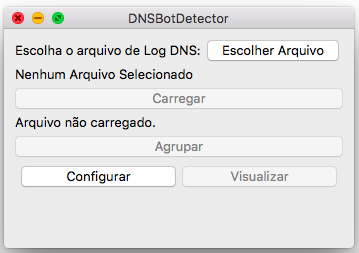
\includegraphics[width=10cm]{initial_screen}
\caption[Tela inicial da Ferramenta]{Tela inicial da Ferramenta} \label{fig:initial_screen}
\end{figure}

Qt é um IDE multi-plataforma que permite desenvolver aplicações com interface gráfica utilizando a linguagem C++ \citep{qtsite}. A escolha de Qt para o desenvolvimento da plataforma foi motivada pelo fato dele ser multi-plataforma, assim como o banco de dados utilizado (PostgreSQL), além do suporte à C++, que foi a linguagem adotada na fase inicial para implementar a preparação de dados.

A aplicação desenvolvida no Qt se comunica com o módulo desenvolvido em Python que serve de interface para leitura do banco de dados até o consumo final dos dados do banco, seja através de planilhas ou gráficos de distribuição espacial. As transações entre o interface gráfica e Python foram todas feitas através de criação de processos paralelos.

Ao longo dessa seção é exibida a documentação das funcionalidades do sistema, além de uma visão geral sobre a aplicação desenvolvida.

\section{Documentação de Casos de Uso}
Nesta seção é mostrada a documentação dos casos de usos atendidos pelo sistema. São 4 casos de uso no total: Carregar Arquivo de Log DNS, Configurar Técnica de Agrupamento, Visualizar Gráfico e Realizar Agrupamento. O diagrama dos casos de usos pode ser visto na Figura \ref{fig:diagram_use_cases}. 

\begin{figure}
\centering
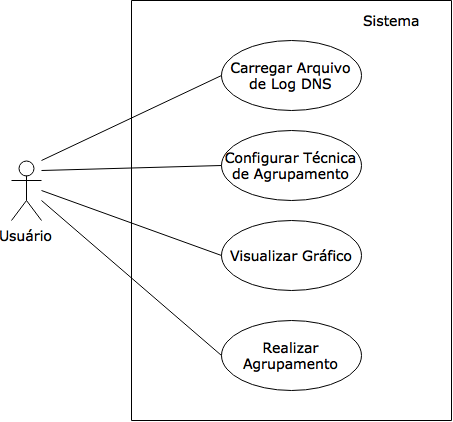
\includegraphics[width=12cm]{diagram_use_cases}
\caption[Diagrama de Casos de Uso]{Diagrama de Casos de Uso} \label{fig:diagram_use_cases}
\end{figure}

A descrição de cada caso de uso é feita ao longo dessa seção. No modelo de especificação de casos de uso utilizado, os passos do Fluxo Básico de Eventos (FBE), são referenciados no Fluxo Alternativo de Eventos. Além disso, as pós-condições são atendidas quando o caso de uso é encerrado com sucesso.

\begin{table}[]
\centering
\caption{Caso de Uso - Carregar Arquivo de Log DNS}
\label{tab:use_case_load_file}
\begin{tabular}{|lp{10cm}|}
\hline
Nome: & Carregar Arquivo de Log DNS  \\ \hline
Ator: & Usuário   \\ \hline
Pré-condições: & Nenhuma   \\ \hline
\multirow{15}{*}{Fluxo Básico de Eventos:} & 1. O Usuário seleciona a opção ``Escolher Arquivo''  \\
 & 2. O Sistema exibe uma janela com os arquivos no formato txt presentes no sistema de arquivos do Usuário.  \\
 & 3. O Usuário seleciona um arquivo de log para importar.  \\
 & 4. O Sistema informa o endereço do arquivo selecionado e disponibiliza a opção ``Carregar''. \\
 & 5. O Usuário seleciona a opção ``Carregar'' \\
 & 6. O Sistema exibe um \textit{pop-up} informando que o arquivo está sendo importado para o banco de dados e inicializa a importação dos dados do arquivo para o banco de dados. \\
 & 7. O Sistema retira o \textit{pop-up} informando que o arquivo está sendo importado para o banco de dados e altera a mensagem ``Arquivo não carregado'' para ``Arquivo de Logs Carregado com Sucesso!'' e o caso de uso é encerrado com sucesso.\\ \hline
\multirow{3}{*}{Fluxo Alternativo de Eventos:} & \textbf{(A1) Nenhum Arquivo Selecionado:} No passo 4 do FBE se nenhum arquivo tiver sido selecionado.\\
 & A1.a) O caso de uso é encerrado com falha.\\ \hline
\multirow{5}{*}{Pós-Condições:} & 1. Os dados contidos no log informado pelo usuário foram carregados no banco de dados. \\
 & 2. As opções ``Agrupar'' e ``Visualizar'' são disponibilizadas.\\
 & 3. A opção ``Carregar'' é desativada.\\
\hline 
\end{tabular}
\end{table}

\begin{table}[]
\centering
\caption{Caso de Uso - Configurar Técnica de Agrupamento}
\label{tab:use_case_config}
\begin{tabular}{|lp{10cm}|}
\hline
Nome: & Configurar Técnica de Agrupamento  \\ \hline
Ator: & Usuário   \\ \hline
Pré-condições: & Nenhuma   \\ \hline
\multirow{12}{*}{Fluxo Básico de Eventos:} & 1. O Usuário seleciona a opção ``Configurar''  \\
 & 2. O Sistema recupera as informações do último arquivo de configuração salvo. \\
 & 3. O Sistema exibe as opções disponíveis para as Informações de Configuração, pré-selecionando as opções recuperadas no passo 2. \\
 & 4. O Usuário seleciona as Informações de Configuração desejadas.  \\
 & 5. O Sistema exclui o arquivo de configuração anterior, salva as Informações de Configuração selecionadas pelo Usuário em um novo arquivo de configuração e o caso de uso é encerrado com sucesso. \\
 \hline
\multirow{9}{*}{Fluxo Alternativo de Eventos:} & \textbf{(A1) Arquivo de Configuração Não Encontrado:} No passo 2 do FBE se o Sistema detectar que o arquivo de configuração anterior não existe.\\
 & A1.a) O Sistema utiliza os valores padrões como informação recuperada do arquivo.\\
 & A1.b) O Sistema retorna ao passo 3 do FBE. \\ 
 & \textbf{(A2) Janela de Configuração Cancelada:} No passo 5 do FBE se o Usuário cancelar a janela de configuração. \\
 & A2.a) O caso de uso é encerrado com falha. \\
 \hline
\multirow{2}{*}{Pós-Condições:} & 1. As Informações de Configuração selecionadas pelo Usuário são armazenadas no arquivo de configuração. \\
\hline
\multirow{10}{*}{Outras Informações:} & 1. Informações de Configuração: Lista de Características para Agrupamento, Algoritmo de Agrupamento e Número de Grupos. \\
 & 2. Valores Padrão: Lista de Características para Agrupamento: [\textit{count\_domain\_with\_numbers, average\_domain\_length, std\_domain\_length, count\_request, average\_requisition\_degree, std\_requisition\_degree, minimum\_requisition\_degree}], Algoritmo de Agrupamento: K-Médias, Número de Grupos: 4. \\
\hline 
\end{tabular}
\end{table}

\begin{table}[]
\centering
\caption{Caso de Uso - Visualizar Gráfico}
\label{tab:use_case_visualize}
\begin{tabular}{|lp{10cm}|}
\hline
Nome: & Visualizar Gráfico  \\ \hline
Ator: & Usuário   \\ \hline
\multirow{2}{*}{Pré-Condições:} & Os dados contidos no log DNS foram carregados no banco de dados.  \\ \hline
\multirow{10}{*}{Fluxo Básico de Eventos:} & 1. O Usuário seleciona a opção ``Visualizar''  \\
 & 2. O Sistema exibe a Lista de Características para Agrupamento disponíveis para serem visualizadas. \\
 & 3. O Usuário seleciona 2 ou 3 características que deseja visualizar em um gráfico e seleciona a opção ``cria gráfico''. \\
 & 4. O Sistema buscará no banco de dados pelos endereços IP e as características selecionadas e apresenta os pontos resultantes em um gráfico e o caso de uso termina com sucesso  \\
 \hline
\multirow{5}{*}{Fluxo Alternativo de Eventos:} & \textbf{(A1) Quantidade de características inválida:} No passo 3 do FBE se o cliente selecionar qualquer quantidade abaixo de 2 e acima de 3.\\
 & A1.a) O Sistema exibe uma mensagem de erro e o caso de uso termina com falha.\\
 \hline
\multirow{2}{*}{Pós-Condições:} & 1. O Sistema exibiu o gráfico interativo com os eixos informados pelo Usuário. \\
\hline
\multirow{5}{*}{Outras Informações:} & 1. Lista de Características para Agrupamento: [\textit{count\_domain\_with\_numbers, average\_domain\_length, std\_domain\_length, count\_request, average\_requisition\_degree, std\_requisition\_degree, minimum\_requisition\_degree}].  \\
\hline 
\end{tabular}
\end{table}

\begin{table}[]
\centering
\caption{Caso de Uso - Realizar Agrupamento}
\label{tab:use_case_clutering}
\begin{tabular}{|lp{10cm}|}
\hline
Nome: & Realizar Agrupamento  \\ \hline
Ator: & Usuário   \\ \hline
\multirow{2}{*}{Pré-Condições:} & Os dados contidos no log DNS foram carregados no banco de dados.  \\ \hline
\multirow{12}{*}{Fluxo Básico de Eventos:} & 1. O Usuário seleciona a opção ``Agrupar''  \\
 & 2. O Sistema apresenta um ambiente para a escolha do destino do arquivo. \\
 & 3. O Usuário escolhe a pasta onde será salvo e o nome do arquivo. \\
 & 4. O Sistema agrupa os IPs segundo suas características resgatadas no banco de dados e aplica um algoritmo de agrupamento com parâmetros definidos no arquivo de configuração.  \\
 & 5. O Sistema salva os IPs e suas características na pasta escolhida pelo usuário e o caso de uso termina com sucesso. \\
 \hline
\multirow{3}{*}{Pós-Condições:} & 1. O arquivo no formato XLS é armazenado no endereço definido pelo Usuário com as informações de cada grupo separadas por aba. \\
\hline
\end{tabular}
\end{table}

\section{Visão Geral do Sistema}
A aplicação desenvolvida serve para auxiliar na detecção de botnets. Esse auxílio é feito baseado em informações coletadas por um servidor de DNS. Para oferecer informações relevantes ao usuário, utilizando os algoritmos de agrupamento, a aplicação segue um fluxo básico, constituídos por etapas distintas: Leitura do Log DNS, Cálculo das Informações dos Domínios, Cálculo das Características das Máquinas, Seleção das Configurações, Execução do Algoritmo de Agrupamento e Disponibilização dos Resultados no Arquivo CSV. A Figura \ref{fig:program_flow} mostra um diagrama do fluxo básico de funcionamento do sistema.

As etapas de Leitura de Log DNS, Cálculo das Informações das Informações dos Domínios e Cálculo das Características são feitas durante o caso de uso descrito na Tabela \ref{tab:use_case_load_file}. Na etapa de Leitura de Log DNS, é feita a extração das informações brutas coletadas pelo servidor DNS para o banco de dados. Nas etapas de Cálculo, as informações são calculadas utilizando chamadas as funções de agrupamento do SQL.

Na Etapa de Seleção das Configurações, descrita pelo caso de uso na Tabela \ref{tab:use_case_config} ...

Por fim, na fase de Execução do Algoritmo de Agrupamento..

%%TODO mostrar telas com estados do Sistema: e.g. layout do xls gerado, pop para selecionar as configurações, etc....

\begin{figure}
\centering
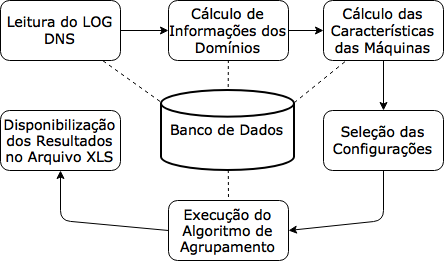
\includegraphics[width=12cm]{program_flow}
\caption[Diagram do Fluxo do Programa]{Diagrama do Fluxo do Programa} \label{fig:program_flow}
\end{figure}
